\section{A counterfactual session-stream experiment}\label{sec:C27:streamcase}
Consider a technical assistant supporting a software team over a sequence of repository tasks. Early sessions establish that one service uses a particular deployment command, that production changes require review, and that a diagnostic document belongs to a restricted project. Later sessions change the command, introduce an exception for a sandbox environment, revoke one user's access, and ask an indirect question whose answer depends on the old experience. The test is not whether the assistant can repeat each fact. It is whether it uses the correct record, scope and authority when choosing an action.

Construct independent task streams from templates with controlled entity substitutions, dependency structures and change schedules. The substitutions prevent exact-string memorization from explaining transfer, while the dependency structure preserves the reasoning required. Separate streams should not share answer-bearing memory unless cross-user sharing is explicitly the treatment. The evaluator retains the authoritative event sequence and can query the environment, but the agent sees only observations available at each step.

Table~\ref{tab:C27:interventions} lists interventions that distinguish the relevant mechanisms. Each row specifies what changes and what observation would diagnose the failure. The table is an experimental design, not a set of reported measurements.
\begingroup\setlength{\tabcolsep}{3pt}\small
\begin{longtable}{L{23mm}L{40mm}L{45mm}}
\caption{Counterfactual interventions in a session stream.}\label{tab:C27:interventions}\\
\toprule Intervention & Controlled change & Diagnostic observation \\
\midrule\endfirsthead
\toprule Intervention & Controlled change & Diagnostic observation \\
\midrule\endhead
Write omission & Remove one source event from the writer input. & A missing record should be attributed to acquisition or writing, not retrieval. \\
Oracle record & Supply the decisive record directly in context. & Continued failure implicates interpretation or action policy under this control. \\
Implicit query & Replace explicit recall wording with a knowledge bridge. & A direct-versus-indirect gap identifies a relevance-routing limitation. \\
Contradiction & Add a newer authoritative correction. & The selected record and action should reflect validity and authority, not mere recency. \\
Scope exception & Make an old procedure valid only in a sandbox. & Blanket reuse or blanket rejection reveals inadequate applicability reasoning. \\
Revocation & Remove a principal's access while paused. & Resumption must not turn historical access into a new authorized effect. \\
Deletion & Remove source content and mark derivatives. & Retrieval and reconstruction should not silently reintroduce excluded information. \\
Migration & Change policy or embedding version at a boundary. & Differences should be linked to representation, retrieval or interpretation changes. \\
\bottomrule\end{longtable}
\endgroup

The baseline conditions should preserve information and budget as carefully as possible. A direct-context oracle can consume more prompt space than a retrieval system, so reserve equivalent context capacity or report the difference. A full-history baseline can become infeasible at long horizons; report the horizon at which it ceases to fit rather than silently switching its truncation policy. A simple raw-log retriever provides an important control because it avoids extraction errors while retaining the same source evidence.

Writer and reader policies should be crossed. A high-quality writer paired with a weak reader may produce accurate records that are misapplied. A strong reader paired with an aggressive summarizer may never receive the decisive constraint. Crossing these components identifies interaction effects and prevents a memory engine from receiving credit for a better backbone. The experiment should also vary whether outcome feedback is gold, self-judged, delayed or unavailable. A method that relies on immediate correct labels has a different deployment requirement from one operating without them.

Task order needs independent replication. Generate several permutations of the same multiset and several independently sampled streams. The first comparison isolates curriculum effects conditional on the tasks; the second supports broader generalization. Preserve the entire evolving memory for each run so failures can be traced to prior updates. Reusing a bank built under one order across all conditions would remove an important source of variation and could favor methods compatible with that bank's organization.

The primary outcomes include verified task completion, constraint adherence, temporal correctness, authorized evidence use and recovery after interruption. Intermediate outcomes include write coverage, retrieval of decisive records, correct rejection of obsolete records and calibrated influence. These outcomes should be linked rather than pooled indiscriminately. For example, a retrieval improvement with no action improvement can reveal a reader bottleneck; an action gain accompanied by unauthorized context use is not an acceptable solution to the stated task.

Negative controls are essential. Include tasks where the remembered deployment command is irrelevant, where the restricted document is unnecessary, and where the sandbox exception should not generalize. Otherwise an agent that always emits warnings or always retrieves every memory can receive undeserved credit. Measure over-application and under-application separately, as motivated by MemCalib, while retaining the end-to-end storage and retrieval components that its supplied-memory setting intentionally isolates.

Failure adjudication should use the event history and artifact state, not the agent's explanation alone. A stored memory can claim that a tool failed because credentials were invalid when the actual cause was a temporary outage. If this explanation becomes a procedural rule, later tasks may avoid a useful tool unnecessarily. The evaluator should identify the original observation, the inferred lesson and the later consequence. This causal chain distinguishes bad experience attribution from simple forgetting.

Finally, report the maintenance workload as the bank grows. Track raw and derived storage, index updates, compaction, merge operations, deletion propagation and retrieval latency. A sublinear skill count does not imply bounded total memory if raw trajectories and subtask nodes continue to grow. Nor does a compact bank guarantee low decision cost if each query invokes extensive reasoning. The study should expose which resource grows with episodes, which is amortized across reuse, and which can be bounded only by discarding information. Those operating conditions determine whether a promising memory mechanism can support sustained agent execution.

The public HyperSkill implementation provides a concrete separation between the hypergraph core and the per-task provider interface\cite{xu2026hyperskill}. A reproduction should instrument both: the core determines candidate reachability and maintenance, while the provider determines when retrieval and ingestion occur relative to task execution. Logging only final skill counts would miss a provider that ingests outcome information too early. Logging only model context would miss a maintenance operation that changes the interpretation of later records. Attach task and memory-version identifiers to each operation so the two traces can be joined.

The implementation audit should also verify that the evaluator's gold outcome is unavailable to deployment-style variants before they commit their own interpretation. A gold-feedback experiment is useful for estimating mechanism potential, but it should not be confused with a self-judged agent. When switching to self-judgment, measure the resulting memory-label errors and their downstream accumulation rather than reporting only final success. A modest immediate error rate can have a disproportionate longitudinal effect if the same mistaken lesson is reused repeatedly.

The fragility study's published code and InMind's released diagnostic resources offer additional primary anchors for this audit\cite{ye2026fragility,inmind2026}. Their existence improves inspectability but does not establish that the experiment described here has run. The appropriate next record is an immutable implementation revision, complete stream manifest and trace of the actual interventions. Until those observations exist, the proposed factorial and counterfactual tests remain a research design with explicit rejection criteria, not evidence of achieved lifelong reliability.

The inspected provider exposes \path{provide_memory} and \path{take_in_memory}; instrumentation at these boundaries can establish whether evidence was supplied before a decision or incorporated only after the task outcome.

\subsection{What a counterfactual replay can identify}\label{sec:C27:counterfactualreplay}
Replaying logged actions under a changed memory policy does not by itself estimate that policy's end-to-end performance. Once a changed context induces another action, the future tool results, environment and memory writes can diverge. Continuing to supply the original observations then evaluates a hybrid trajectory that neither policy would necessarily generate. The problem is particularly acute for recoverable effects: an original successful write cannot be assumed to exist after a counterfactual policy chose a read instead.

A frozen-prefix test can legitimately compare next-action distributions from the same recorded state, provided both contexts contain only information available at that boundary. This identifies local sensitivity, such as whether a revoked instruction changes a proposal, rather than full task success. A full counterfactual test must rerun the environment from a valid checkpoint or use a justified transition model, exposing model error and replay limits. Importance weighting requires logged behavior probabilities and support for the alternative actions; deterministic tool logs do not supply those conditions automatically. Thus paired prefix diagnostics, complete reruns and model-based counterfactuals should be reported as distinct evidence products rather than interchangeable forms of replay.


Figure~\ref{fig:C27:overview} isolates the mechanism and its stated information boundaries.
\begin{figure}[!htbp]
\centering
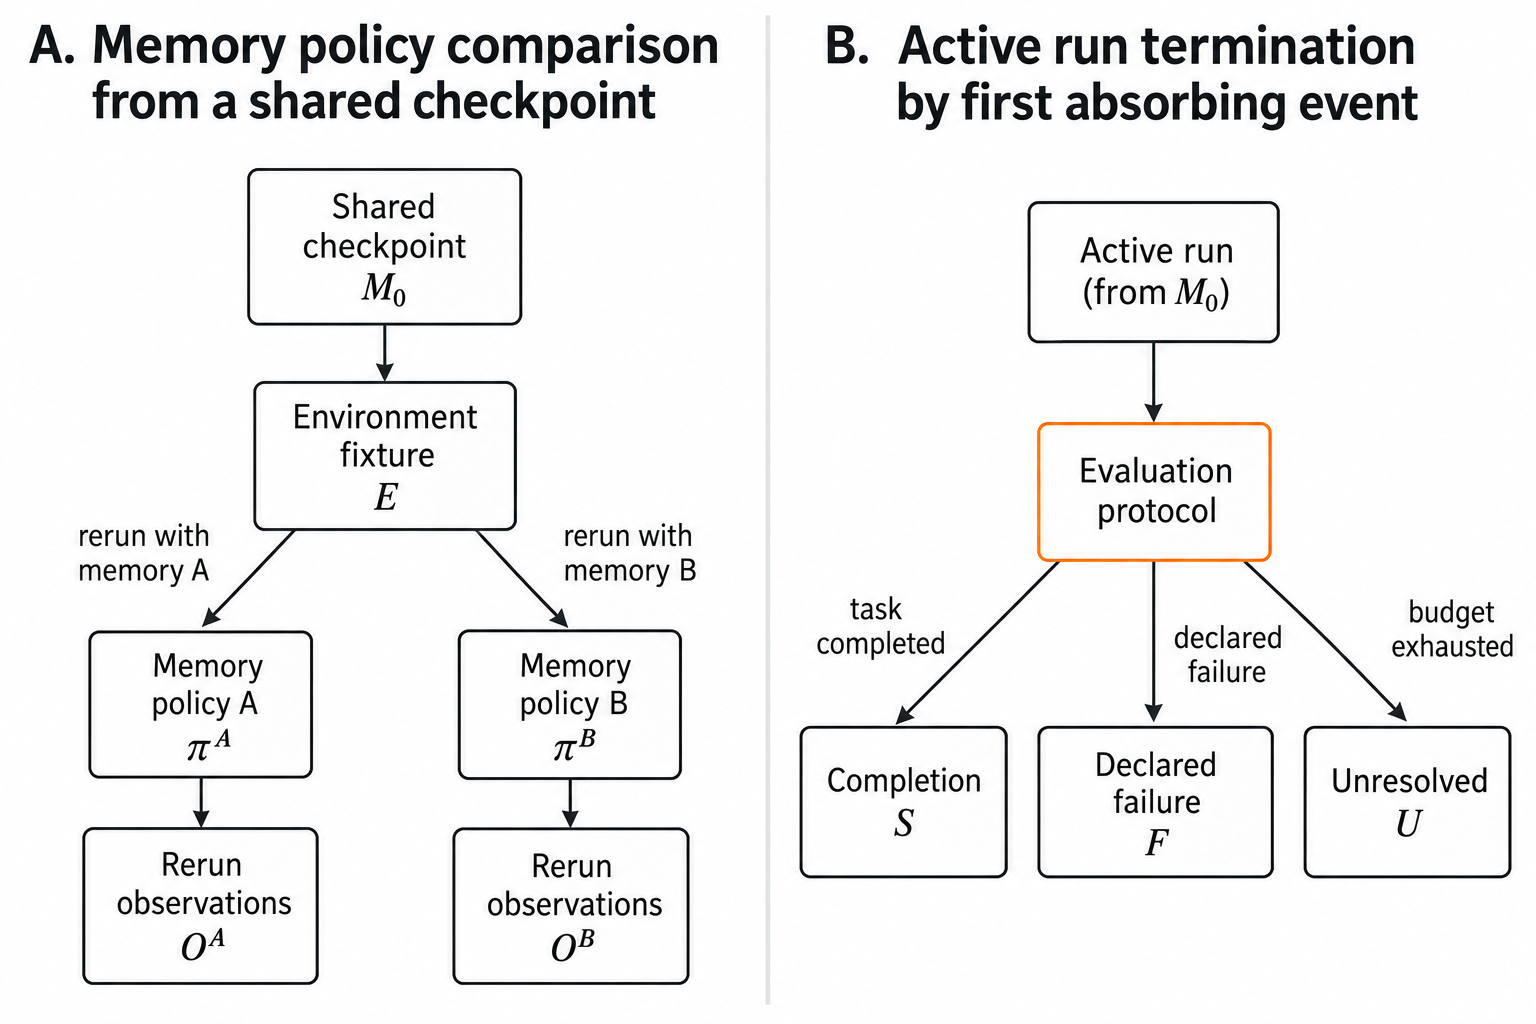
\includegraphics[width=\linewidth]{book/figures/assets/F27review.png}
\caption{Memory policies $\pi^A,\pi^B$ share an initial fixture $(M_0,E)$ but can produce different rerun observations $O^A,O^B$. Observation-changing counterfactuals require valid reruns, not substituted answers on one fixed log. Completion $S$, declared failure $F$ and unresolved budget stops $U$ are distinct protocol outcomes; interpreting a stop as censoring requires additional assumptions. The figure-local S/F/U labels name outcome categories, not stopping times.}
\label{fig:C27:overview}
\end{figure}
